%% ===============================================================================================
%% @author Leonardo Florez-Valencia (florez-l@javeriana.edu.co)
%% @author David Enrique Palacios García (david_palacios@javeriana.edu.co)
%% @author Karen Sofía Coral Godoy (corallg_ksofia@javeriana.edu.co)
%% ===============================================================================================

\documentclass[letter]{article}

\usepackage[spanish]{babel}
\usepackage[margin=1in]{geometry}
\usepackage{amsmath}
\usepackage{amsthm}
\usepackage{amssymb}
\usepackage[utf8]{inputenc}
\usepackage{graphicx, color}
\usepackage{algorithm}
\usepackage{algpseudocode}
\usepackage{mathrsfs}
\graphicspath{ {graphics/} }
% Some definitions
\floatname{algorithm}{Algoritmo}

% Author info
\title{Escritura del problema de la representación binaria inversa}
\author{David Enrique Palacios García$^1$ \and Karen Sofia Coral Godoy$^1$}
\date{
	$^1$Departamento de Ingeniería de Sistemas, Pontificia Universidad Javeriana\\Bogotá,  Colombia \\
	\texttt{\{david\_palacios, corallg\_ksofia\}@javeriana.edu.co}\\~\\
	\today
}

\begin{document}
\maketitle
	
\begin{abstract}
En este documento se presenta la formalización del problema de la inversión de una cadena, junto con la descripción de dos algoritmos que lo solucionan. Además, se presenta un análisis experimental de la complejidad de esos dos algoritmos.
\textbf{Palabras clave:} inversión, algoritmo, formalización, experimentación, complejidad, cadena.
\end{abstract}

\tableofcontents
\newpage
	
\section{Introducción} \label{intro}
Invertir una cadena puede llegar a ser útil para encontrar similitudes entre datos, tal así, que existe un gran número de formas para hacerlo. El ejemplo práctico que se tratará en este documento será tomar un número natural N, convertirlo a cadena binaria, invertir esta cadena y, finalmente, obtener el valor entero de la cadena invertida. Para resolver este problema se presentan dos algoritmos que lo solucionan, con el objetivo de mostrar: la formalización del problema (sección \ref{formalizacion}), la escritura formal de ambos algoritmos (sección \ref{algoritmos}) y un análisis experimental de la complejidad de cada uno de ellos (sección \ref{experimentos}).

\section{Formalización del problema} \label{formalizacion}
Cuando se piensa en {\it invertir una cadena} la solución inmediata puede ser muy simplista: inocentemente, se piensa en leer una cadena de atrás hacia adelante. Sin embargo, con un poco más de reflexión, hay tres preguntas que pueden surgir:
\begin{enumerate}
  \item ¿Cadena es únicamente de tipo \texttt{String}?
  \item ¿Cómo se guardan esas cadenas en memoria?
  \item ¿Solo se pueden ordenar letras?
\end{enumerate}

Recordemos que, en memoria, una cadena de tipo \texttt{String} es un arreglo de datos de tipo caracter. Además, es necesario entender que cualquier caracter utilizado por una máquina en realidad tiene un valor \texttt{ASCII}. Esto significa que cualquier letra, símbolo o número representado por una máquina, se puede escribir como una secuencia de caracteres.
Basado en esta premisa, entendemos que convirtiendo cualquier dato en un arreglo de caracteres, podemos invertir su secuencia y obtener un nuevo dato.

\subsection{Definición del problema de la ``inversión de la cadena''} \label{problema}
Así, el problema de invertir se define a partir de:
  \begin{enumerate}
    \item una secuencia $S$ de elementos $a\in \mathbb{N}$
  \end{enumerate}
producir una nueva secuencia $S'$ cuyos elementos cumplan con la relación $a_n,~ a_{n-1},~ ...~ a_0$.
\begin{itemize}
    \item Entradas:
    \begin{itemize}
        \item $S = \left< a_i \in \mathbb{N} \right> ~ | ~ 1\le i \le n$.
    \end{itemize}
    \item Salidas:
    \begin{itemize}
        \item $S' = \left< e_i \in S m\right> ~ | ~ e_n,~ e_{n-1} \forall i \in \left[1,n\right)$.
    \end{itemize}
\end{itemize}

\section{Algoritmos de solución} \label{algoritmos}
\subsection{Iterativo}
\label{algoritmos:iterativo}
La idea de este algoritmo es: invertir la cadena recorriendo todos elementos desde la última hasta la primera posición.
\newpage

\begin{algorithm}[!htb]
\caption{Binario inverso Iterativo: Convertir un entero a cadena de caracteres binarios}
\begin{algorithmic}[1]
\Require $n \in \mathbb{N} $
\Procedure{DecimalToBinary}{$n$}
 \State {$binary  \leftarrow [*]char$}
 \State{$i \leftarrow 0$}
  \While{$n != 0$}
    \State{$i \leftarrow i+1$}
     \State {$binary[i]  \leftarrow \texttt{$(char)$}(n \%2) $}
     \State {$n \leftarrow \Call{Floor}{n/2}$}
  \EndWhile
  \State \textbf{return} $binary$
\EndProcedure
\end{algorithmic}
\end{algorithm}

\begin{algorithm}[!htb]
\caption{Binario inverso Iterativo: Invertir una cadena de caracteres}
\begin{algorithmic}[1]
\Procedure{InvertChain}{$S$}
 \If{$|S| = 1$}
      \State \textbf{return} $S[1]$
      \EndIf

  \State {$inverted  \leftarrow [*]char$}
 \For{$i \leftarrow |S|~\mathbf{to}~1~\mathbf{step}~-1$}
      \State {$inverted[i]  \leftarrow S[i] $}
    \EndFor
  \State \textbf{return} $inverted$
\EndProcedure
\end{algorithmic}
\end{algorithm}


\begin{algorithm}[!htb]
\caption{Binario inverso Iterativo: Convertir una cadena de caracteres binarios a un entero}
\begin{algorithmic}[1]
\Ensure $n \in \mathbb{N} $
\Procedure{BinaryToDecimal}{$binary$}
 \State {$decimal \leftarrow 0$}
 \State{$i\leftarrow0$}
 \State{$invertedChain \leftarrow \Call{InvertChain}{binary}$}
 \For{$i, \leftarrow 1~\mathbf{to}~ |invertedChain|$}
  \State {$p \leftarrow \Call{Pow}{(int)invertedChain[i]*2,i}$}
  \State{$decimal\leftarrow decimal+p$}
      
    \EndFor
  \State \textbf{return} $decimal$
\EndProcedure
\end{algorithmic}
\end{algorithm}




\subsubsection{Análisis de complejidad} \label{algoritmos:inocente:complejidad}

Por inspección de código: Se puede observar que, cada paso de la resolución del problema tiene un único ciclo, por lo que la complejidad de cada uno es $O(n)$. Vale la pena resaltar que el algoritmo que realmente nos interesa es el \texttt{Algoritmo 2}, pues es quien invierte cualquier cadena. El \texttt{Algoritmo 1 y 3} realmente son auxiliares para esos sub-problemas (convertir enteros a binarios y viceversa) en particular.

\newpage

\subsubsection{Invariante} \label{algoritmos:inocente:invariante}

Después de cada iteración controlada, el elemento $i$ queda en el lugar invertido que le corresponde, es decir $|S|-1$.

\begin{enumerate}
    \item Inicio: $i=0$, la secuencia vacía está invertida.
    \item Iteración: $1 \le i<|S|$, si se supone que los $i-1$ elementos ya están en su posición, entonces la nueva iteración llevará los $i$-ésimo elementos a su posición adecuada, es decir al inicio de la secuencia.
    \item Terminación: $i=0$, los $|S|$ elementos están en su posición, entonces la secuencia está invertida completamente.
\end{enumerate}


\subsection{Dividir y vencer} \label{algoritmos:dyv}
La idea de este algoritmo es: en primera medida, entender que la inversión de una cadena con un único elemento, es igual a la cadena inicial, este siendo el caso base. Por otra parte,
eligiendo un pivote en el medio de la secuencia, permite dividirla en subsecuencias de carácteres, que a su vez, son invertidas de derecha a izquierda. Para este caso, también se cuenta con los \texttt{algoritmos 1 y 3}, para convertir números enteros a cadenas binarias y viceversa.


\begin{algorithm}[!htb]
\caption{Binario inverso DyV}
\begin{algorithmic}[1]
\Procedure{InvertChain}{$S, l, r$}
\If{$l=r$}
      \State \textbf{return} $S[i]$
      \EndIf
 \State {$q  \leftarrow \Call{Floor}{(l+r)/2}$}
 \State {$left  \leftarrow$} \Call{InvertChain}{S,l,q} 
 \State {$right  \leftarrow$}
 \Call{InvertChain}{S,q+1,r}
 \State {$result  \leftarrow [*]char$}
 \For{$i \leftarrow 1~\mathbf{to}~|right|$}
      \State {$result[i] \leftarrow (right[i]) $}
    \EndFor
    
     \For{$i \leftarrow 1~\mathbf{to}~|left|$}
      \State {$result[i]  \leftarrow (left[i]) $}
    \EndFor
  \State \textbf{return} $result$
\EndProcedure
\end{algorithmic}
\end{algorithm}

\subsubsection{Análisis de complejidad} \label{algoritmos:inocente:complejidad}

El algoritmo ¨InvertChain de dividir y vencer¨ tiene orden de complejidad $O(1)$ cuando hay un elemento en la secuencia $S$, es decir $n=1$.\\
     \\
     Cuando $n>1$ la complejidad del algoritmo según el teorema maestro está dada por:
    
     \begin{equation}
T(n)= 2T\  \frac{n}{2} + O(n)
\end{equation}
    
El valor de $a = 2$\\
El valor de $b = 2$\\
La complejidad de $C(n) = O(n)$\\
    
Esto resulta en un órden de complejidad similar a \texttt{MergeSort}, con una complejidad de $O(n)$ para su función auxiliar. Esto hace que la complejidad algorítimica de este algoritmo sea $O(nlogn)$; siendo más lento que su contraparte iterativa.

\subsubsection{Invariante} \label{algoritmos:inocente:invariante}

La invariante esta dada por: en cada paso de división se realiza el intercambio de la secuencia desde el pivote hacia los extremos.

\section{Análisis experimental} \label{experimentos}

En esta sección se presentarán los resultados del experimento para confirmar los órdenes de complejidad de los dos algoritmos presentados en la sección \ref{algoritmos}.

\subsection{Múltiplos de 10} \label{experimentos:aleatorias}

Acá se presentan los experimentos cuando los algoritmos se ejecutan con números que son múltiplos de 10, es decir, si contiene a 10 varias veces exactamente. Además, en cada iteración cada número va incrementando en un digito.

\subsubsection{Protocolo}
\begin{enumerate}
    \item Definir una muestra de 8 números, cada número debe incrementar en un digito a el anterior respectivamente.
    \item Cada algoritmo se ejecutará 10 veces con cada número y se guardará el tiempo promedio de ejecución.
    \item Se genera el gráfico necesario para comparar los algoritmos.
\end{enumerate}

\subsubsection{Experimentación}
\begin{enumerate}
    \item Se utilizó el programa \texttt{$run\_experiment.cpp$} el cual internamente define los 8 números requeridos, que son:
    \begin{itemize}
        \item \texttt{10,340,1890,14870,354880,1254690,78465460,988641540} 
    \end{itemize}
    \item El programa logró finalizar sin complicaciones, con un tiempo expresado en segundos.
    \item Se obtuvieron los mismos 8 datos con el tiempo promedio de cada uno de los algoritmos (Ver tabla 1), logrando así crear la siguiente gráfica: (ver Figura 1)
\end{enumerate}

\begin{figure}[h]
    \centering
    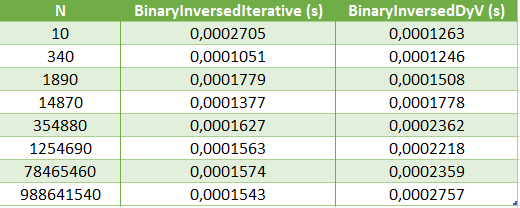
\includegraphics[scale=1]{Data.png}
    \label{experimentos:aleatorias:grafica}
    
\end{figure}



\begin{figure}[h]
    \centering
    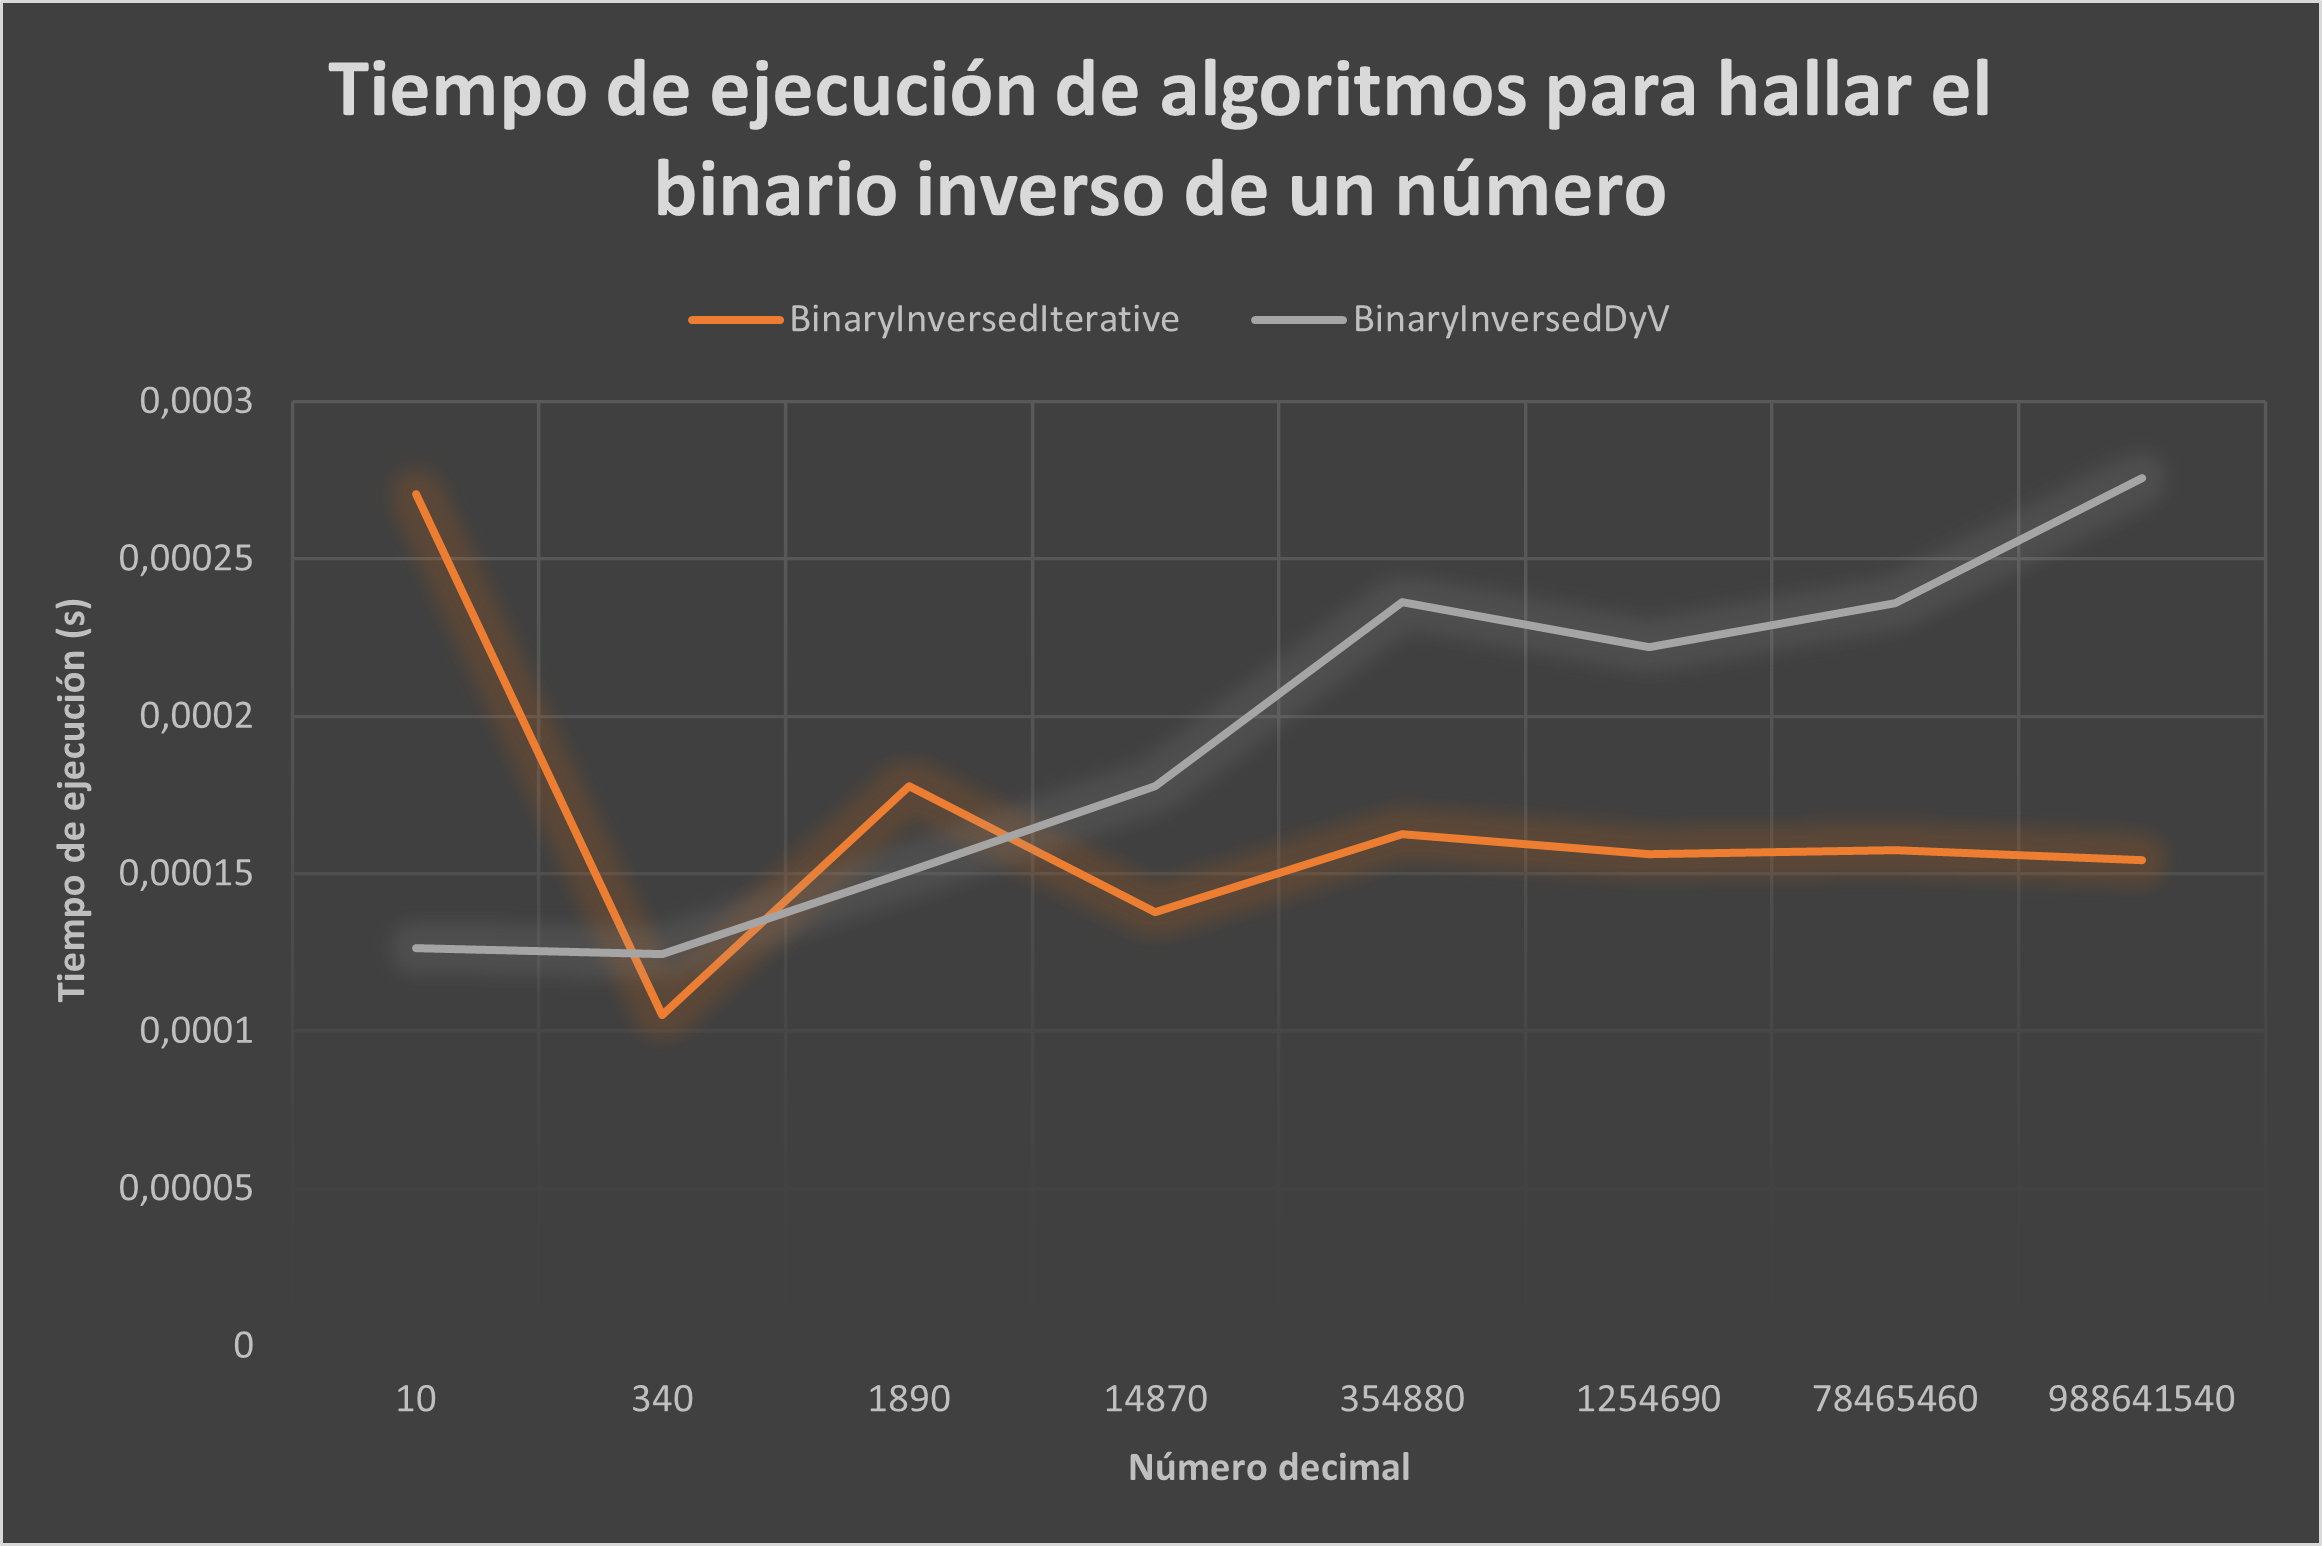
\includegraphics[scale=0.76]{DataGraphic.png}
    \label{experimentos:aleatorias:grafica}
    \caption{Tiempo de ejecución de los algoritmos}
\end{figure}

\subsubsection{Análisis del experimento}
\label{experimentos:aleatorias:analisis}
Como se expreso previamente, el algoritmo iterativo tiene una complejidad $\Theta(n)$ y el algoritmo de dividir y vencer tiene una complejidad $\Theta(nlogn)$, por lo que se asume que el algortimo más rápido es el iterativo, sin embargo, a partir del segundo número múltiplo de 10 seleccionado, se empieza a notar esto. Por el contrario, para el caso del primer número no se cumple, puesto que el $\log(n)$ siendo $n \leq 10$ dará como resultado un número $\leq 1$ para finalmente reducir el tiempo de ejecución del algortimo de dividir y vencer sobre el iterativo. Para los números $> 10$ el tiempo del algoritmo iterativo será menor, como se esperaba, al hallar las complejidades de cada algoritmo. 

\section{Conclusiones}
El experimento fue útil para concluir:
\begin{enumerate}
    \item El tiempo de ejecución para el caso promedio del algoritmo planteado de dividir y vencer tiene una complejidad igual al algoritmo de \texttt{MergeSort} siendo $\Theta(nlogn)$ 
    \item Aunque se plantee un algoritmo de dividir y vencer, no implica que sea el adecuado para solucionar el problema.
    \item Para determinar si un algoritmo es más rápido que otro, debe evaluarse cada caso individualmente, aunque su orden de complejidad sea menor no garantiza que en todos los casos el tiempo también lo sea. 
\end{enumerate}




\end{document}

%% eof - main.tex
